\documentclass[12pt,parskip=full]{article}
\usepackage{lmodern}
\usepackage{amsmath}
\usepackage[left=1.0in,right=1.0in,top=1.0in,bottom=1.0in]{geometry}
\geometry{letterpaper}
\usepackage{graphicx}
\usepackage{caption}
\usepackage{subcaption}
\usepackage{longtable}
\usepackage{float}
\usepackage{wrapfig}
\usepackage{soul}
\usepackage{textcomp}
\usepackage{marvosym}
\usepackage{wasysym}
\usepackage{latexsym}
\usepackage{amssymb}
\usepackage{apacite}
\usepackage{tabu}
\usepackage[svgnames]{xcolor}
\usepackage{tikz}
\usepackage[linktoc=all]{hyperref}
\usepackage{cleveref}
\usepackage{listings}
\usepackage{setspace}
\usepackage{parskip}
\usepackage{array}
\usepackage{apacite}
\usepackage{natbib}
\usepackage{multicol}
\usepackage{subcaption}
\usetikzlibrary{arrows}

\pgfdeclarelayer{edgelayer}
\pgfdeclarelayer{nodelayer}
\pgfsetlayers{edgelayer,nodelayer,main}

\tikzstyle{none}=[inner sep=0pt]
\tikzstyle{waypt}=[circle,fill=Black,draw=Black,scale=0.4]
\tikzstyle{Helobody}=[circle,fill=White,draw=Black,scale=4.0]
\tikzstyle{Tailrotor}=[circle,fill=White,draw=Black,scale=1.0]
\tikzstyle{ForceVector}=[->,draw=Indigo,fill=Indigo]
\tikzstyle{Coordinate}=[->,draw=Red,fill=Red,fill opacity=1.0]
\tikzstyle{angle}=[->]
\tikzstyle{MeasureMark}=[|-|]
\newlength{\imagewidth}
\newlength{\imagescale}

\setlength{\parskip}{11pt}
%\setlength{\parindent}{15pt}
\usepackage{bookmark}
\makeatletter
\renewcommand\@seccntformat[1]{}
\makeatother

\lstset
{
    language=Matlab,
    keywords={break,case,catch,continue,else,elseif,end,for,function,
        global,if,otherwise,persistent,return,switch,try,while},
    basicstyle=\ttfamily,
    keywordstyle=\color{blue},
    commentstyle=\color{ForestGreen},
    stringstyle=\color{purple},
    numbers=left,
    numberstyle=\tiny\color{gray},
    stepnumber=1,
    numbersep=10pt,
    backgroundcolor=\color{white},
    tabsize=4,
    showspaces=false,
    showstringspaces=false
}

\newcommand{\Lagr}{\mathcal{L}}

\renewcommand{\thesection}{\arabic{section}}

\renewcommand{\thesubsection}{\thesection\alph{subsection}}
\renewcommand{\theequation}{\thesection.\arabic{equation}}

\numberwithin{subsection}{section}

\begin{document}
	\vspace{-2ex}
	\title{Report 4\vspace{-3.5ex}}
	\author{Rob Rau\vspace{-4ex}}
	\date{\today\vspace{-4ex}}
	\maketitle

	\section{First, the Easy Stuff}
		
		Given the function
		\begin{equation}
			f(x) = x_1^2 - x_2
		\end{equation}
		and constraints
		\begin{eqnarray}
			c_1(x) &=& 2x_1 - x_2 \geq 0 \\
			c_2(x) &=& x_1 + x_2 - 1 \geq 0
		\end{eqnarray}
		the Lagrangian takes the form of
		\begin{equation}
			\Lagr(x_1, x_2, \lambda_1, \lambda_2, s_1, s_2) = 
				f(x_1, x_2) - \left(\lambda_1\left[c_1(x_1, x_2) - s_1^2\right] + 
				\lambda_2\left[c_2(x_1, x_2) - s_2^2\right]\right)
		\end{equation}
		which can be expanded to
		\begin{equation}
			\Lagr(x_1, x_2, \lambda_1, \lambda_2, s_1, s_2) = 
				x_1^2 - x_2 - \left(\lambda_1\left[2x_1 - x_2 - s_1^2\right] + 
				\lambda_2\left[x_1 + x_2 - 1 - s_2^2\right]\right)
		\end{equation}

		The following 6 equations can be set up to solve for all 6 unknowns:
		\begin{eqnarray}
			\frac{\partial\Lagr}{\partial x_1} &=& 2x_1 - 2\lambda_1 - \lambda_2 = 0 \\
			\frac{\partial\Lagr}{\partial x_2} &=& \lambda_1 - \lambda_2 - 1 = 0 \\
			\frac{\partial\Lagr}{\partial \lambda_1} &=& 2x_1 - x_2 - s_1^2 = 0 \\
			\frac{\partial\Lagr}{\partial \lambda_2} &=& x_1 + x_2 - 1 - s_2^2 = 0 \\
			\frac{\partial\Lagr}{\partial s_1} &=& \lambda_1 s_1 = 0 \\
			\frac{\partial\Lagr}{\partial s_2} &=& \lambda_2 s_2 = 0
		\end{eqnarray}

		When solved for, there are 5 possible solutions
		\begin{center}
			\begin{tabular}{| c || c | c | c | c | c | c |}
				\hline
				  & $x_1$ & $x_2$ & $\lambda_1$ & $\lambda_2$ & $s_1$ & $s_2$ \\ \noalign{\hrule height 2pt}
				1 & 1 & 2 & 1 & 0 & 0 & $\sqrt{2}$ \\ \hline
				
				2 & 1 & 2 & 1 & 0 & 0 & $-\sqrt{2}$ \\ \hline
				
				3 & 1/3 & 2/3 & 5/9 & -4/9 & 0 & 0 \\ \hline
				
				4 & -1/2 & 3/2 & 0 & -1 & $\frac{i\sqrt{10}}{2}$ & 0 \\ \hline
				
				5 & -1/2 & 3/2 & 0 & -1 & $-\frac{i\sqrt{10}}{2}$ & 0 \\ \hline
			\end{tabular}
		\end{center}

		To fully satisfy the first order KKT conditions $\lambda_k \geq 0$. This leaves only the first and second
		solution as possible optimal solutions. Just by observation we see both solutions are identical as $s_2$
		is squared in the Lagrangian. 

		To determine positive definiteness of the Hessian of the Lagrangian, the active constraint must satisfy
		$\nabla c_k^T(x^*)y = 0$ for some $y \neq 0$. For this solution the only active constraint is $c_1$, so
		\begin{equation}
			\nabla c_1^T(x^*)y = \begin{bmatrix} 2 & -1 \end{bmatrix} \begin{bmatrix} y_1 \\ y_2 \end{bmatrix} = 0
		\end{equation}
		Just by inspection, we can see that $y_1 = 1$ and $y_2 = 2$, thus satisfying the second order conditions
		for a constrained problem.
		
		Therefore the optimal point of the constrained problem is $x^* = \begin{bmatrix} 1 & 2 \end{bmatrix}$.
		
	\section{Now for the Hard Stuff}
	
		\subsection{Logarithmic Interior Penalty}
			The logarithmic penalty function, conceptually isn't to difficult to implement. The core of my implementation
			is the BFGS optimizer I wrote for assignment 3, completely unmodified. The line search that BFGS uses did
			need to be modified somewhat to better handle the infinite values seen with the logarithmic penalty. This
			modification simply made it backtrack if infinity was found.
			
			The other issue I had was when the start point happened to be outside of the feasible region. This would
			cause the line search to choke, as all it saw were infinite values, it didn't have anyplace to go. To
			solve this, I simply performed a line search on the constraint function in the direction of steepest ascent.
			This would move the start point into the feasible region, and the BFGS optimizer would handle it from there.
			I do not know how this method would work when there are multiple constraints. I did not have time to study
			this. If I were to hazard a guess, I would try averaging the gradients of each constraint and use that as
			the search direction instead.
			
			When toying around with this optimizer I found two things had the largest effect on the convergence rate.
			The initial size of $\mu$ and how fast $\mu$ is decreased. The larger the initial $\mu$ more major
			iterations are needed to converge. On the surface this doesn't sound ideal, but the fact of the matter is
			that the interior penalty method is an algorithm layered on top of two more algorithms. I found that some
			of the larger initial $\mu$ values were actually better for the underlying BFGS implementation. I imagine
			this is problem dependent, and would probably need to be tuned for different problem spaces.
			
			Changing how much $\mu$ was decreased seemed to have the largest effect. I found that decreasing $\mu$
			a large amount each iteration, in general, would allow for much faster convergence. If, however, $\mu$
			got to small to fast, it would start to cause problems for the BFGS optimizer. Another thing I noticed
			was that this method has a constant number of major iterations regardless of start point.
			
			The interior penalty method ended up converging on the point $AR = 13.60185$ and $S_{ref} = 12.54455$
			with a drag value of $D = 258.74594N$.
		
		\subsection{Sequential Quadratic Programming}
		
			We can see from the result given by the interior penalty method, that the constraint was active. Because
			of this, we can treat that inequality constraint as an equality constraint to use with the SQP method.
			
			I found SQP to be more robust than the interior penalty method. It took less fussing around with parameters
			to achieve good results. It is also much faster than the interior penalty method. I found that on average it
			would take more major iterations to converge, it still spent much less computational time to find the result.
			The reason for this is because the SQP algorithm does not spend nearly as much time in minor iterations. I
			found that, for this problem at least, the line search in SQP was almost never run. This will most likely
			not be the case with a different problem set, but for this one it seems to be.
			
			The obvious disadvantage SQP has is that it is only built to handle equality constraints without major
			modifications. This also means that it does not have the same problem that the interior penalty method
			has when starting outside of the feasible region.
			
			The following plots show the paths of travel for both the interior penalty method as well as SQP.
			\begin{figure}[!ht]
				\centering
				\begin{subfigure}[h]{0.45\textwidth}
					\includegraphics[width=\textwidth]{Opt1.eps}
					\subcaption{Drag minimization with start point of $AR = 48$, $S_{ref} = 52$}
				\end{subfigure}
				\begin{subfigure}[h]{0.45\textwidth}
					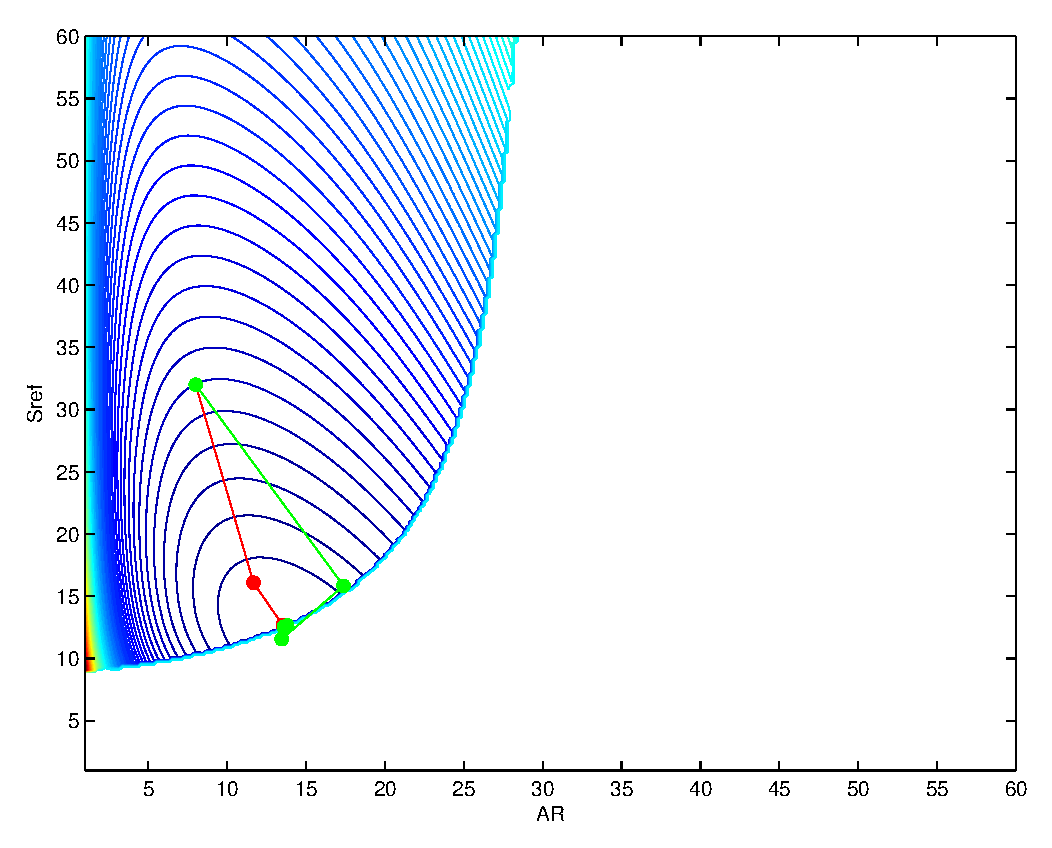
\includegraphics[width=\textwidth]{Opt2.eps}
					\subcaption{Drag minimization with start point of $AR = 8$, $S_{ref} = 32$}
				\end{subfigure}
				\begin{subfigure}[h]{0.45\textwidth}
					\includegraphics[width=\textwidth]{Opt3.eps}
					\subcaption{Drag minimization with start point of $AR = 28$, $S_{ref} = 10$}
				\end{subfigure}
				\caption{Comparison logarithmic interior penalty and SQP\label{fig:paths}}
			\end{figure}
			As \cref{fig:paths} shows, SQP first couple of moves take it to the equality constraint. From there
			it follows the constraint until it finds the minimum point.
			
			While SQP is faster than the interior penalty method, it has some major drawbacks. The fact that it
			can't handle inequality constraints was already mentioned, but further than that theres the fact
			that it does spend more time outside of the feasible region than the interior penalty method. This
			means that if the simulation is needed to be stopped early, the solution may be infeasible.
			
	\section{Final Thoughts}
	
		Both methods have their merits. SQP is fast, but only for equality constraints, while interior penalties
		are slower, but work with inequalities and guaranty feasibility.
		
		I also learned an import lesson about the complex step derivative method. When trying to debug why my
		optimizers would go off in the weeds, I discovered that when they would travel into negative values for
		$AR$ and $S_{ref}$ the drag function would produce imaginary numbers due to the square roots involved in
		the computing the span of the wing. This caused the complex step method to produce garbage results and 
		thus threw the optimizers off. One needs to be careful when using the complex step method as to not fall
		into the same trap I did. 
		
\end{document}
























